% !TEX root = ./master.tex
 
\section{Results and Discussion}

\subsection{Classification Methods }

\subsection{Data Representation}

\subsection{Classification of Individual Tweets}
\begin{figure*}[t]
	%\vskip -0.2in
	%\begin{center}
	\centering
		\centerline{
			\subfigure[IMDB ]{
				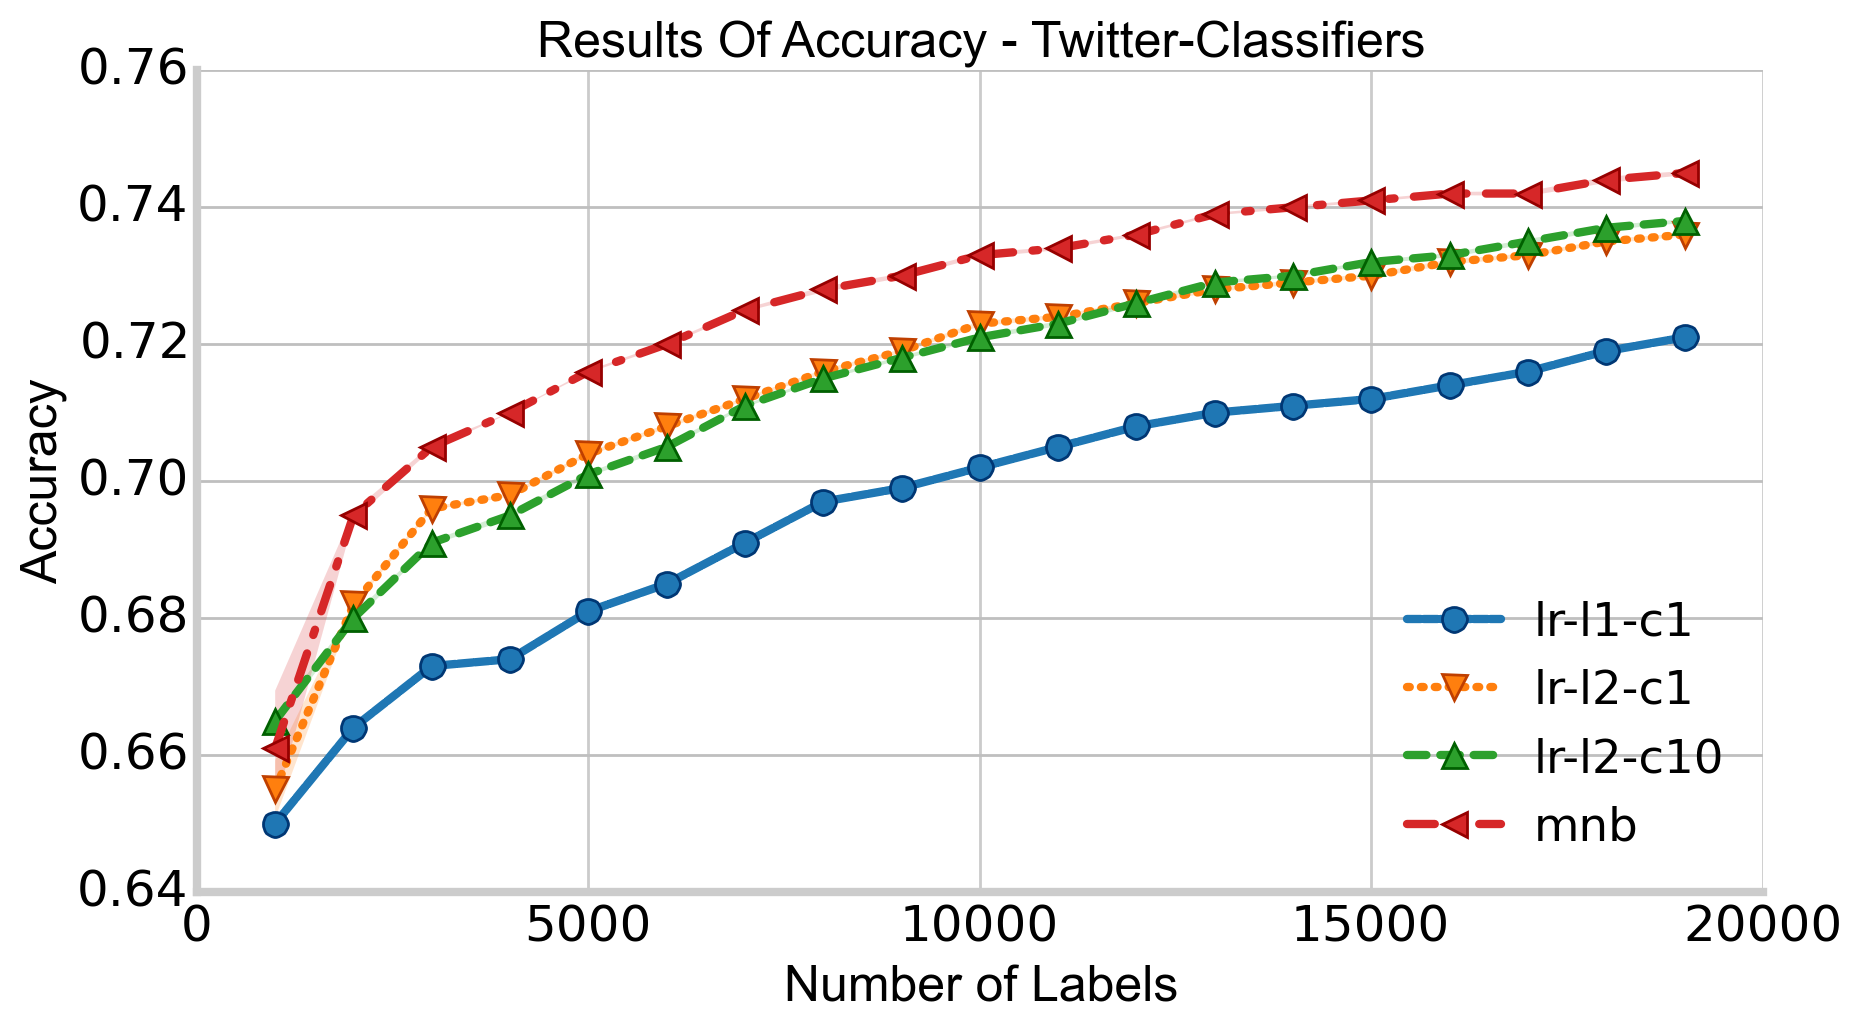
\includegraphics[width=0.7\columnwidth]{fig/twitter-classifiersaccuracy.png}
			\label{fig:class}	
			}	
		}
		\vskip -0.15in
		\caption{Classification models induced on tweets.}
		\label{fig:user}
	%\end{center}
	\vskip -0.1in
\end{figure*}

\begin{figure*}[t]
	%\vskip -0.2in
	%\begin{center}
	\centering
		
			\subfigure[IMDB ]{
				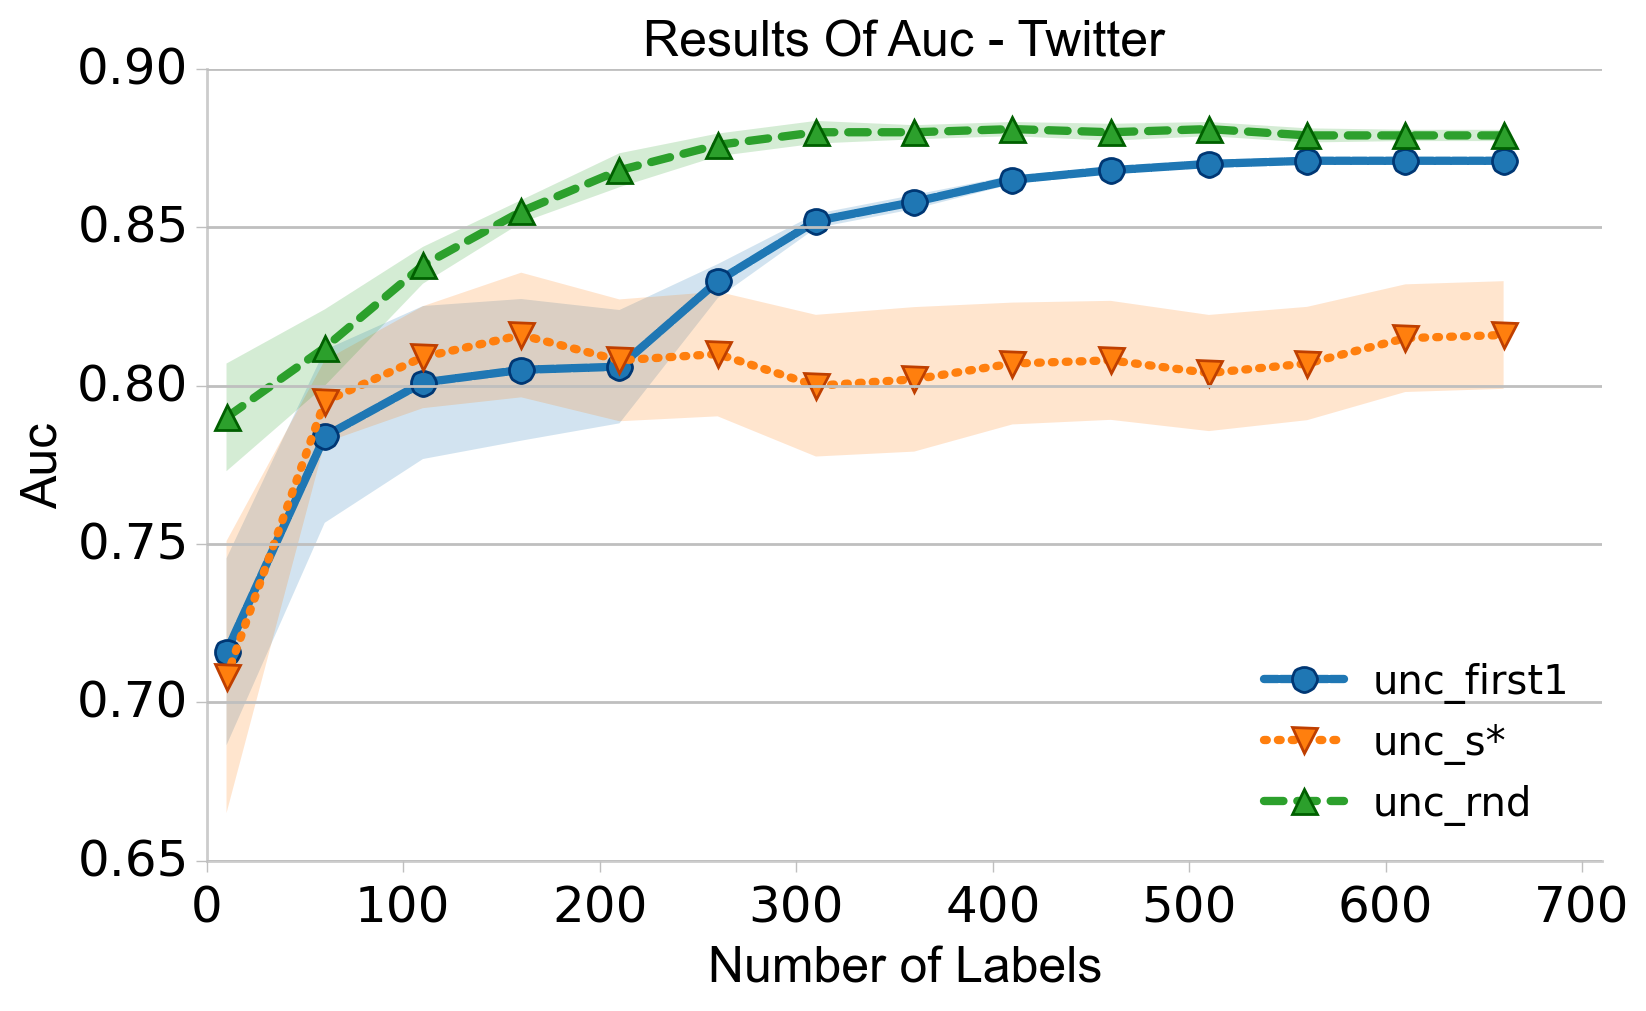
\includegraphics[width=0.7\columnwidth]{fig/twitterauc.png}
			\label{fig:class}	
			}	
		
		\vskip -0.15in
		\caption{Active Learning.}
		\label{fig:user}
	%\end{center}
	\vskip -0.1in
\end{figure*}


\subsection{Bootstrap Effect}
\begin{figure*}[t]
	%\vskip -0.2in
	%\begin{center}
	\centering
		
			\subfigure[IMDB ]{
				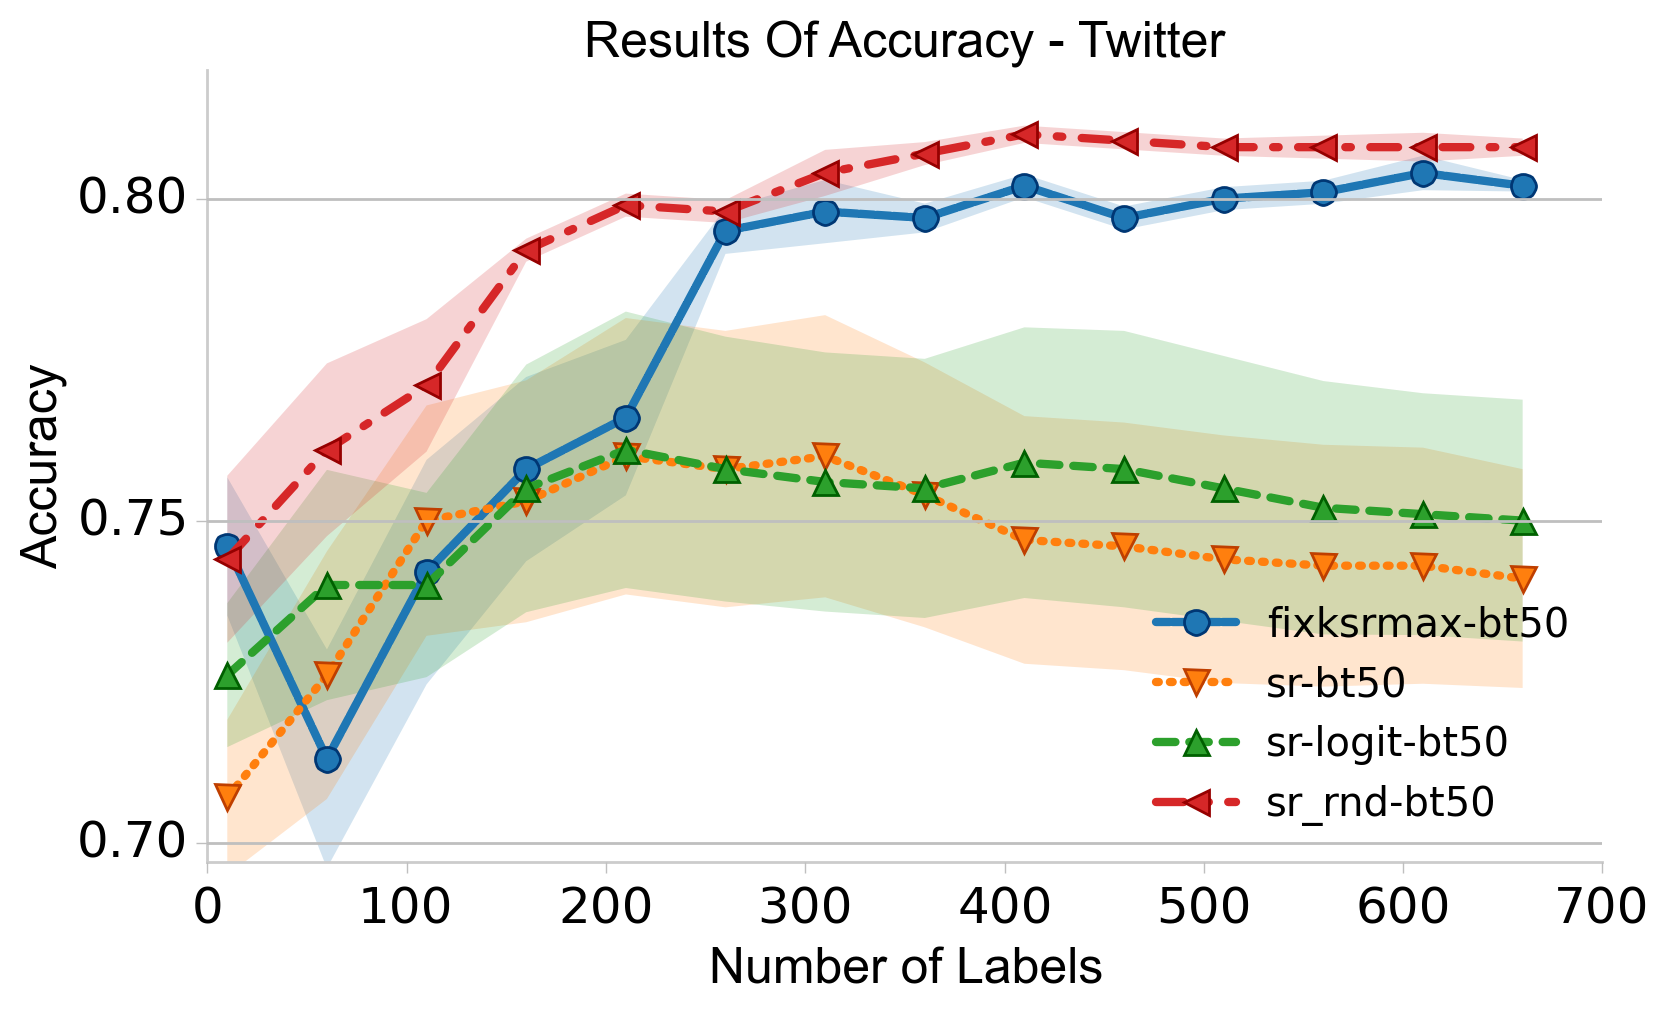
\includegraphics[width=0.7\columnwidth]{fig/twitteraccuracy.png}
			\label{fig:class}	
			}	
		
		\vskip -0.15in
		\caption{Active Learning.}
		\label{fig:user}
	%\end{center}
	\vskip -0.1in
\end{figure*}
\subsection{calibration effect}

\begin{figure*}[t]
	%\vskip -0.2in
	%\begin{center}
	\centering
		
			\subfigure[IMDB ]{
				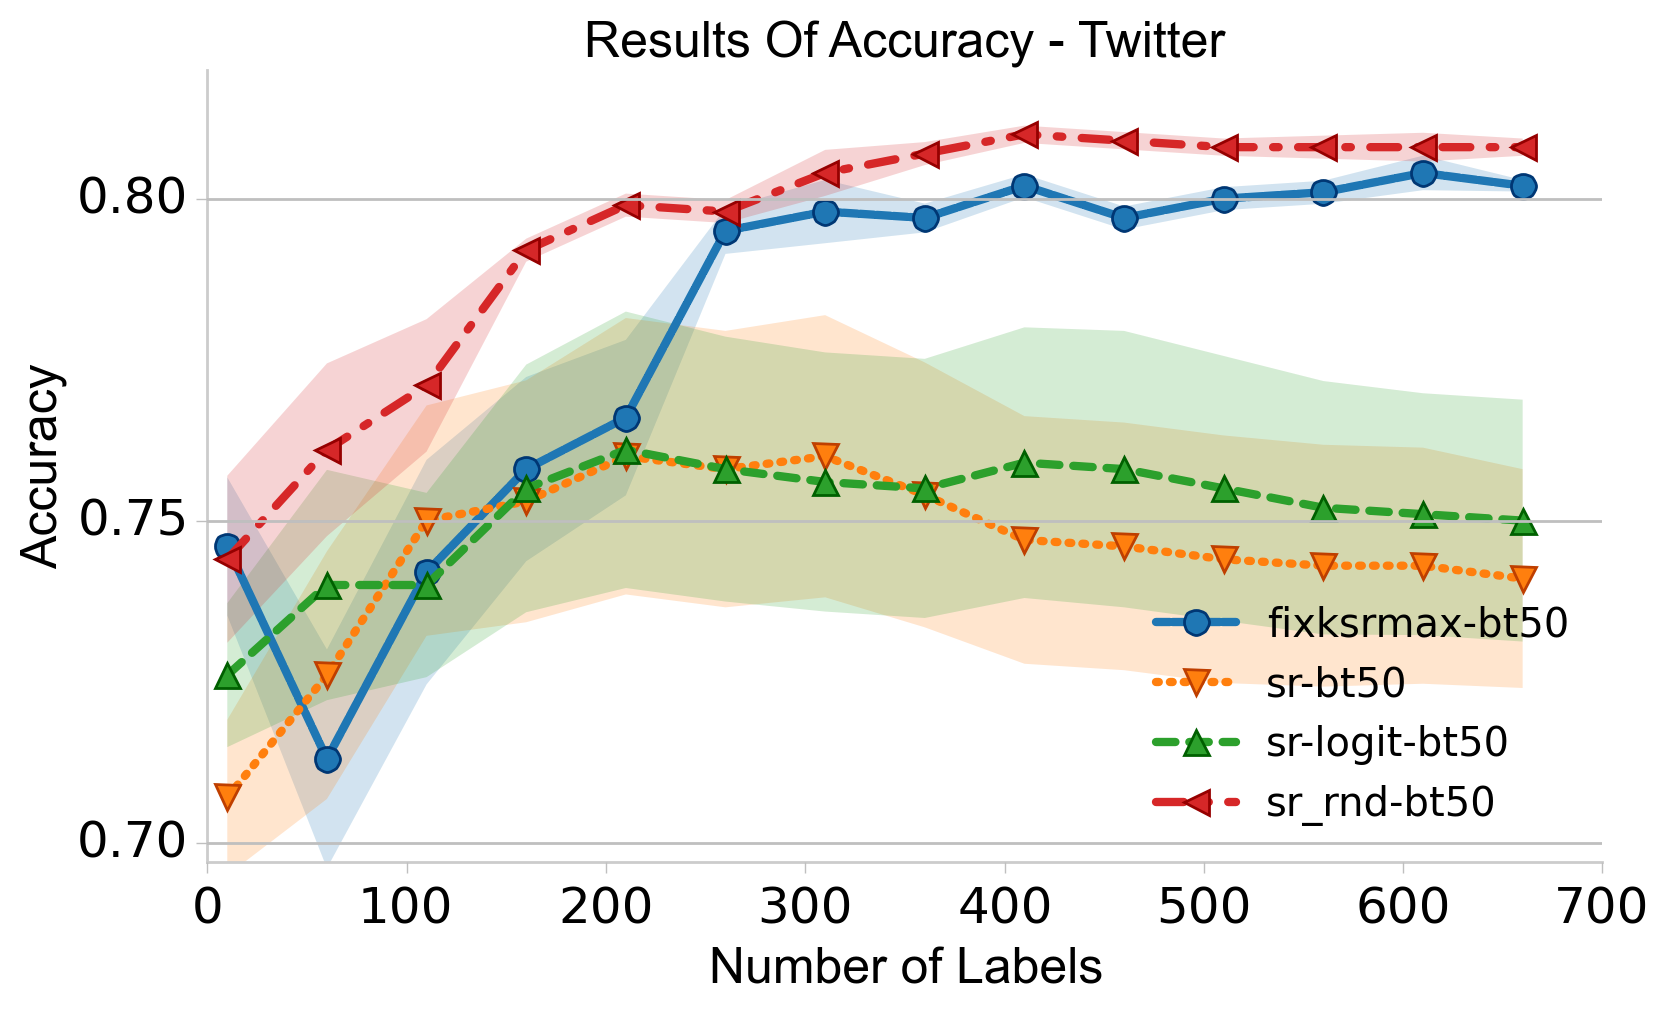
\includegraphics[width=0.7\columnwidth]{fig/twitteraccuracy.png}
			\label{fig:class}	
			}	
		
		\vskip -0.15in
		\caption{\fixme{Active Learning.}}
		\label{fig:user}
	%\end{center}
	\vskip -0.1in
\end{figure*}